\documentclass[a4paper, 12pt]{article}

% Document
\usepackage[utf8]{inputenc}
\usepackage[swedish]{babel}
\usepackage{parskip}
\usepackage{pdfpages}
%\usepackage{apa6}
\usepackage[margin=1in]{geometry}

% Equations
% \usepackage{amsmath}
% \usepackage{siunitx}

% Graphics
\usepackage{graphicx}
% \usepackage{tikz}

% Tables
\usepackage{booktabs}
\usepackage[tableposition=top]{caption}

% References
\usepackage{apacite}
\usepackage{url}
%\usepackage{hyperref}

\begin{document}
\pagenumbering{gobble} % Remove page numbering

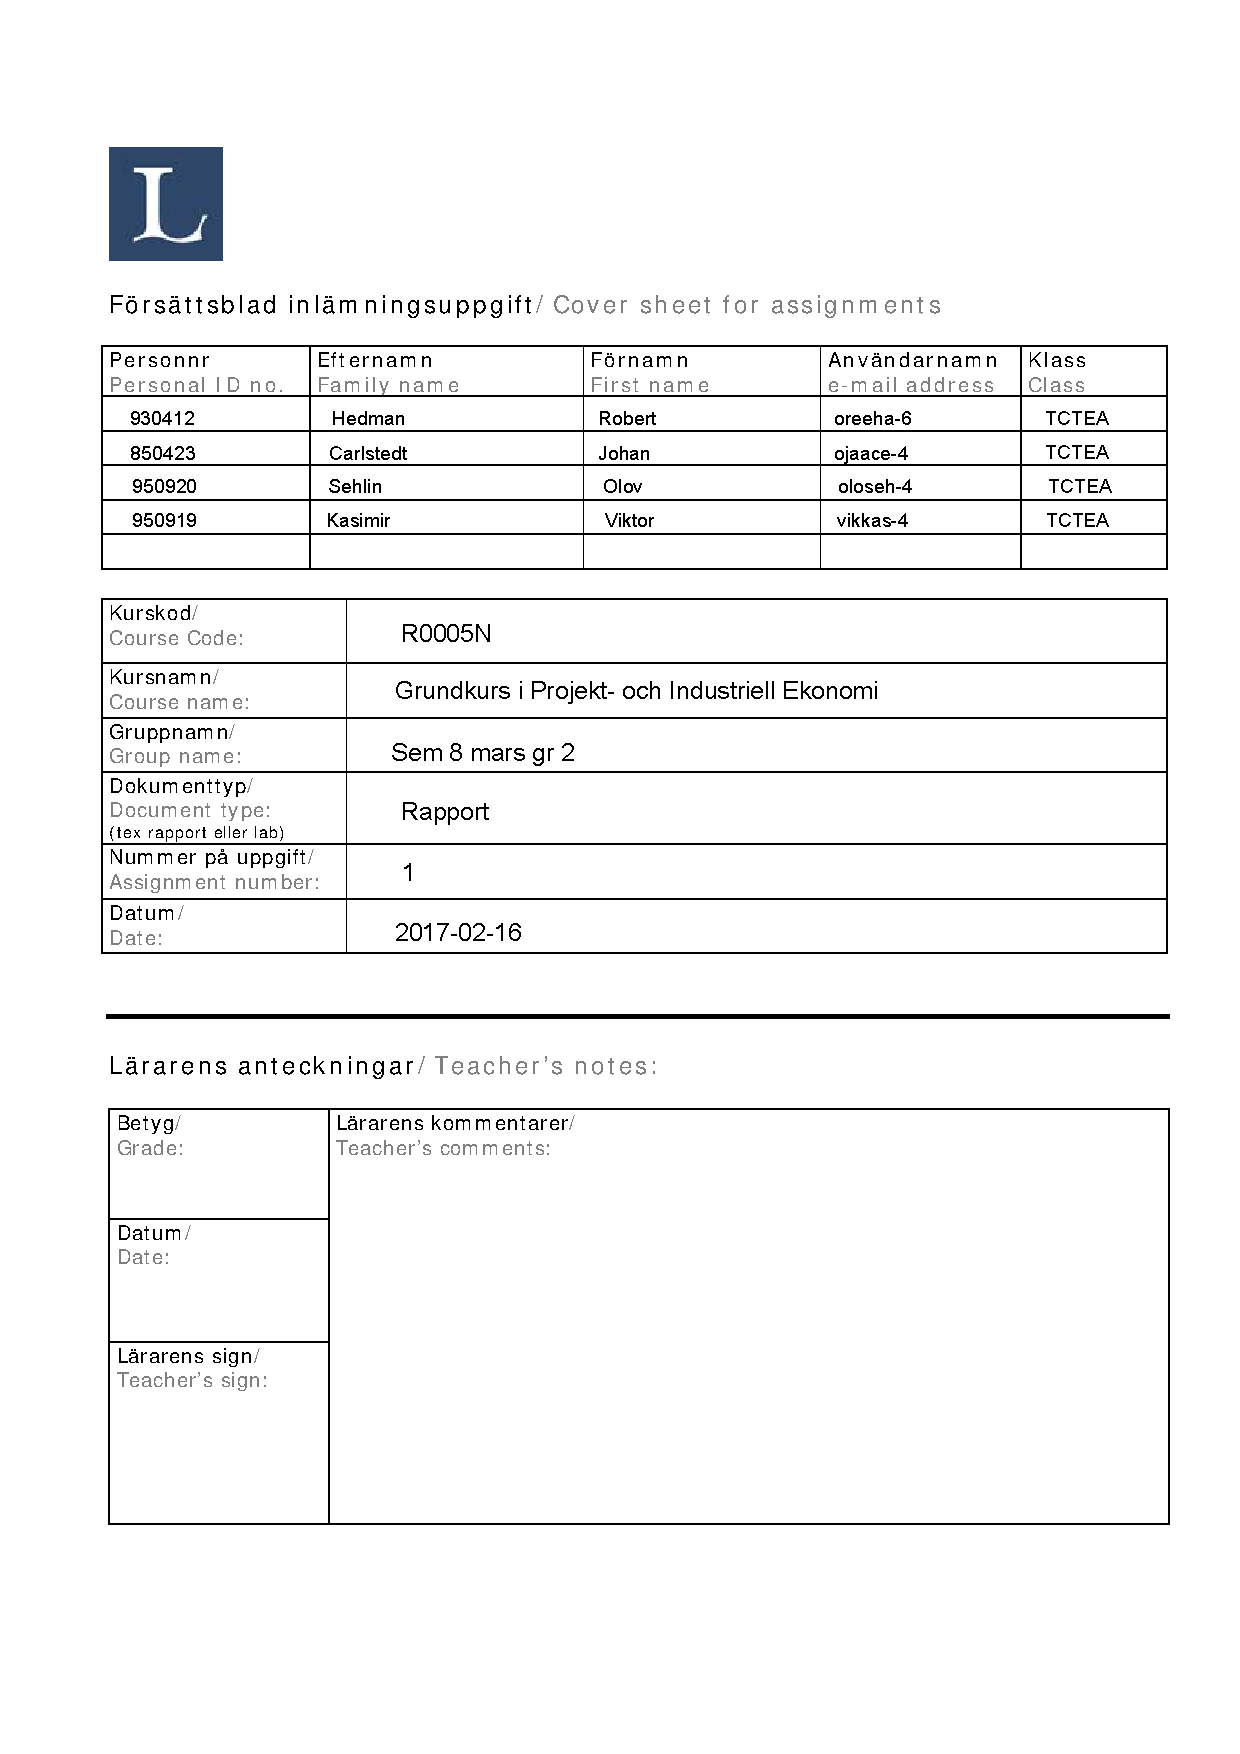
\includepdf{inc/front.pdf}

\tableofcontents
\newpage

\pagenumbering{arabic} % Start page numbering

\section{Introduktion}
För att erhålla insikter lämpliga för en ingenjör om ekonomistyrning har produktkalkylens betydelse och användning inom ett företag som tillämpar kalkylen dagligen undersökts.
Det finns även andra typer av styrmedel, men vid inledande kontakt med företaget föreslogs det från företagets sida att man kunde undersöka produktkalkyl då stor kompetens inom just det området fanns.
Teori har lagts sida vid sida med hur det fungerar i praktiken och undersökts.
Företaget som undersökts är MacGregor.
MacGregor tillverkar och utvecklar bland annat lyftkranar av ett brett sortiment och rekommenderade oss att intervjua dom om just produktkalkylen då den är vital för deras företagande.


% Syfte: Att erhålla insikter om ekonomistyrning så som den används i praktiken
% Erhålla insikter mellan relationen om hur det fungerar i verkligheten, vad vi får läsa i kursen, osv.
% Öva/planera/genomföra projektarbete samt att skriva en rapport

%
%   MÅL
%

% \subsection{Mål?}
% \begin{itemize}
%     \item Beskriv vad som vi vill uppnå med denna rapport/uppgift
% \end{itemize}

%
%   BAKGRUND
%

%       ###################################
%       #             Robert              #
%       ###################################
\subsection{Bakgrund} 
Företag behöver generellt sett ha en budget.
För att kontrollera budgeten används ekonomiska styrmedel.
En form av styrmedel kallas för självkostnadskalkyl.
För att få en uppfattning om företagets ekonomiska situation samt göra kloka beslut inför framtiden används diverse olika kalkyler.
En självkostnadskalkyl är den övergripande termen som beskriver metoden att fördela ett företags kostnader på godtyckliga kostnadsbärare.
Resultatet från en självkostnadskalkyl kan sedan användas som styrmedel för företagets ekonomiska framtid.
Ett exempel av en självkostnadskalkyl är produktkalkyl.
I en produktkalkyl är kostnadsbäraren företagets produkter och alla kostnader fördelas på dessa.
Varianter på produktkalkyler inkluderar påläggskalkyl, bidragskalkyl samt ABC-kalkyl.

Företag, som har en försäljning av varor, får en stor fördel av att använda en produktkalkyl eftersom man snabbt kan se om en produkt är lönsam eller inte.
Eftersom civilingenjörer ofta är med och tar fram och/eller utvecklar nya produkter är denna form av kalkyl en av de första ingenjörer kommer i kontakt med.
En grundläggande förståelse för dessa typer av kalkyler underlättar då kommunikation med ekonomiavdelningen på ett företag; vi som utbildar oss till civilingenjörer drar nytta av att fördjupa oss i denna kalkyl. 

Ett företag som tillämpar produktkalkyl, har stor vikt vid deras ingenjörer och som var villiga att ställa upp på en intervju var Macgregor. 
Vid inledande kontakt med företaget föreslogs det från företagets sida att man kunde undersöka produktkalkylen ABC-kalkyl då stor kompetens inom just det området fanns.


%generell ABC kalkyl och hur den arbetas med.

I en ABC-kalkyl fördelas inte företagets kostnader ut på de färdiga produkterna direkt utan kostnadsbärarna är aktiviter.
Namnet kommer från engelskans {\bf A}ctivity {\bf B}ased {\bf C}osting.


% \begin{itemize}
%     \item Vad är en produktkalkyl?
%     \item Varför valde vi produktkalkyl?
%     Vid inledande kontakt med företaget föreslogs det från företagets sida att man kunde undersöka produktkalkyl då stor kompetens inom just det området fanns.
%     Eftersom civilingengörer ofta blir projektledare lär vi ganska snabbt komma i kontakt med produktkalkylen. Att förstå denna underlättar kommunikation med överorndnade samt styret.
%     \item Hur arbetar man generellt med en sådan? Med hjärnan.
% \end{itemize}


%
%   TIDSPLAN
%

\subsection{Tidsplan}
\begin{table}[ht]
    \centering
    \caption{Tidsplan med datum och aktivitet för projektet}
    \label{tidsplan}
    \begin{tabular}{lllll}
        31/1 & Inledande kontakt med MacGregor via mail    \\
        2/2 & Gruppmöte för planering av projekt    \\
        7/2 & MacGregor godkände samabete med projektet    \\
        9/2 & Gruppmöte för planering av intervju    \\
        10/2 & Första intervjun med MacGregor via Skype   \\
        15/2 & Gruppmöte för planering av rapportskrivande    \\
        16-17/2 & Eventuell andra intervjun med MacGregor via Skype   \\
        17/2 & Macgregor läser igenom repporten   \\
        20/2 & Inlämning av rapport   \\
        24/2 & Gruppmöte för planering av återkoppling av annan rappport    \\
        27/2 & Inlämning av återkoppling av annan rapport  \\
        6/3 & Gruppmöte för planering av seminarium    \\
        8/3 & Seminarium
    \end{tabular}
\end{table}
\begin{itemize}
    \item En tabell med vilka tider vi hade intervjuer.
    \item Tipunkter när vi samlades och diskuterade saker.
    \item Tidpunkter när vi ska vara klara med vissa delar av arbetet. osv...
    \item Hur vi planerade intervjuerna, varför vi planerade för 2st.
\end{itemize}

%       ###################################
%       #            End Robert           #
%       ###################################


\newpage
\section{Resultat}
Ein stein liten sak \cite{dne}.

Nu kollar vi nästa cite \cite{macgregor}.

%
%   INTERVJU 1
%

\subsection{Intervju 1}
\begin{itemize}
    \item Vad fick vi ut från intervju 1? Svar på frågor
\end{itemize}
Oj oj oj.
Vi fick dom bästa svaren!
Dom absolut bästa!
Och du ska veta, du ska veta, jag känner till bra svar!
När jag säger att vi fick bra svar så betyder det att vi fick bra svar!
Gör Afrika bra igen!

%
%   INTERVJU 2
%

%\subsection{Intervju 2}
%\begin{itemize}
%    \item Vad behövde kompleteras från intervju 1?
%\end{itemize}

\newpage
\section{Diskussion}
Ej klar ännu. 
Ingen ny information om företaget kommer att presenteras här.

% %
% %   JÄMFÖRELSE
% %

% \subsection{Jämförelse Förväntningar - Resultat?}
% \begin{itemize}
%     \item Är produktkalkylen rättvisande för produkten de säljer?
%     \item Var det som vi förväntade oss?(Jämför bakgrund och resultat, alltså hur det generellt fungerar och hur företaget faktiskt jobbar med det.)
% \end{itemize}

% %
% %   ARBETSSÄTT
% %

% \subsection{Arbetsätt}
% \begin{itemize}
%     \item Är företagets sätt att hantera deras produktkalkyl något bra?
% \end{itemize}

% %
% %   FÖRBÄTTRINGAR
% %

% \subsection{Förbättringar}
% \begin{itemize}
%     \item Finns det något som kan göras bättre? (som vi kan se)
% \end{itemize}

\newpage
\bibliographystyle{apacite}
\bibliography{ref}
\appendix
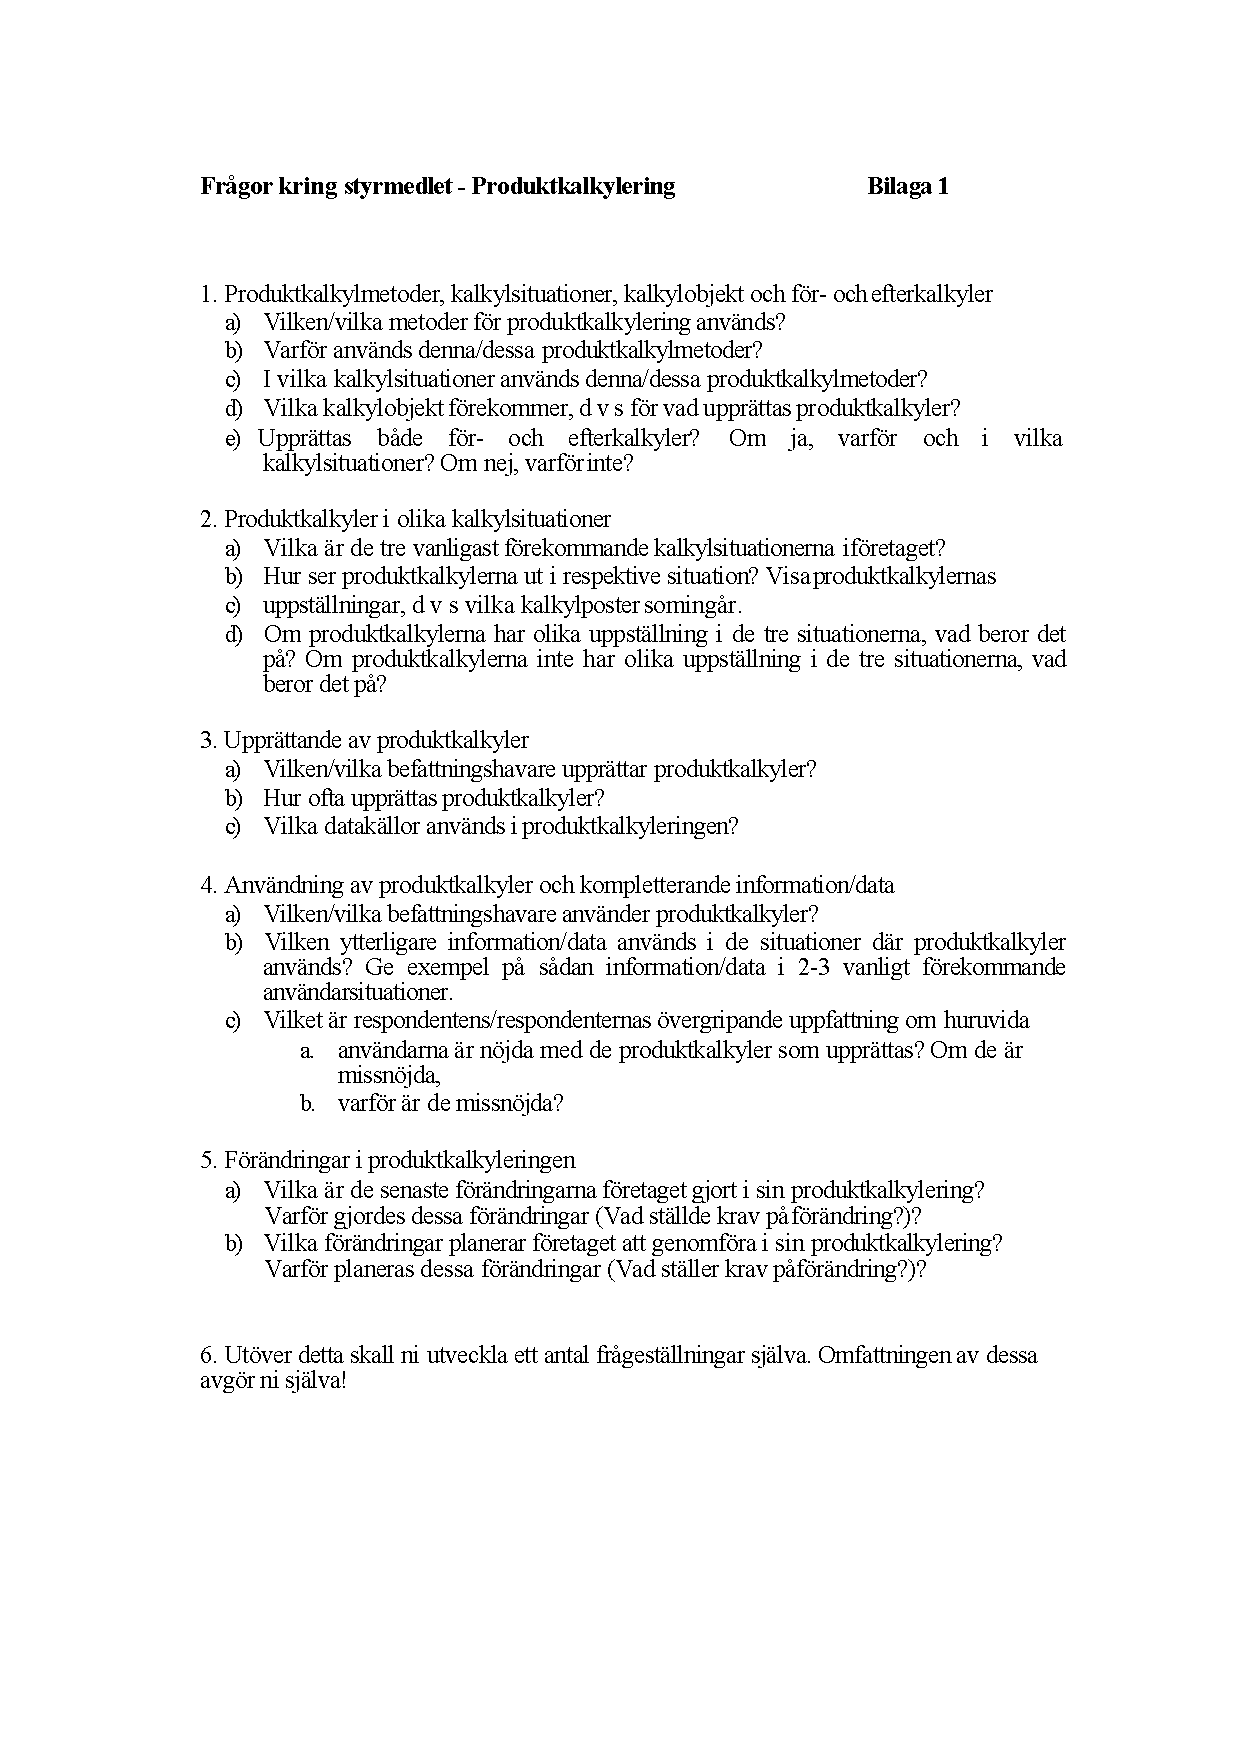
\includepdf[pages=1,scale=.9,pagecommand={\section{Frågor till intervju om produktkalkyl}\label{apdx:fragor}},linktodoc=true]{inc/fragor.pdf}
\end{document}